\section{Time Projection Chamber -- GridPix, Bonn}
\subsection{Introduction}
The project studies the pixelized readout of a TPC for the ILD detector. The readout is based on the Timepix ASIC with a triple GEM or Micromegas based gas amplification.

\subsection{Recent Milestones}
The first studies were based on the triple GEM setup with a single Timepix chip. This readout was mounted in a small test detector in the Bonn laboratory. Here, the working principle was tested with a long drift distance. It could be demonstrated that the transverse spatial resolution of the reconstructed primary electrons was close to the expected diffusion limit of single electrons. The results are summarized in the following publications:
\begin{itemize}
\item \fullcite{6359808}
\item \fullcite{4774978}
\item \fullcite{1748-0221-4-11-P11015}
\item \fullcite{Kaminski:2010zzc}
\item \fullcite{Schade2011128}
\end{itemize}

The new focus are GridPix based detectors, where the gas amplification stage is a Micromegas produced in a postprocessing technique, which guarantees a high quality grid well aligned with the readout pixels. This approach was pioneered by NIKHEF and the University of Bonn has modified the production process together with the Fraunhofer Institut IZM so that a wafer-based production of GridPix detectors is standard by now. The new GridPixes were tested on small prototype detectors and also assembled in an 8 GridPix module for the Large Prototype detector at DESY. A successful test beam campaign was performed last year.
\begin{itemize}
\item \fullcite{1748-0221-9-01-C01033}
\item \fullcite{Koppert2013245}
\end{itemize}
The current work is focused on a new LP module with about 160 GridPixes. The central module is equipped with 96 GridPixes and the two outer modules have 32 GridPixes arranged to maximize the lever arm. This setup serves a demonstrator that larger areas (~$\unit[400]{cm^2}$) can be produced and operated. It was tested in the Large Prototype of the LCTPC collaboration in March/April of 2015 and operated for more than one week permanently in the test beam. A total of about 200 runs with more than 1.5 million events were recorded.
For this a number of challenges had to be overcome. In particular commercial readout systems are not easily scalable. This is why Bonn has developed a cheap and easily expandable system based on the Scalable Readout System (SRS) of the RD51 collaboration.

In addition Bonn is developing the software for reconstructing and analyzing the test beam and simulation data. For this the LCTPC software framework of MarlinTPC is used.
\begin{itemize}
\item \fullcite{4774731}
\end{itemize}

Finally, Bonn also takes part in designing new pixel chips. To test the new digitization and readout techniques two test chips were designed in collaboration with N'IKHEF. Then Bonn also contributed to the design of the Timepix successor chip, Timepix3, which is being tested now:
\begin{itemize}
\item \fullcite{1748-0221-5-12-C12005}
\item \fullcite{6748097}
\item \fullcite{1748-0221-9-01-C01052}
\end{itemize}

\begin{figure}
	\begin{minipage}{.49\textwidth}
		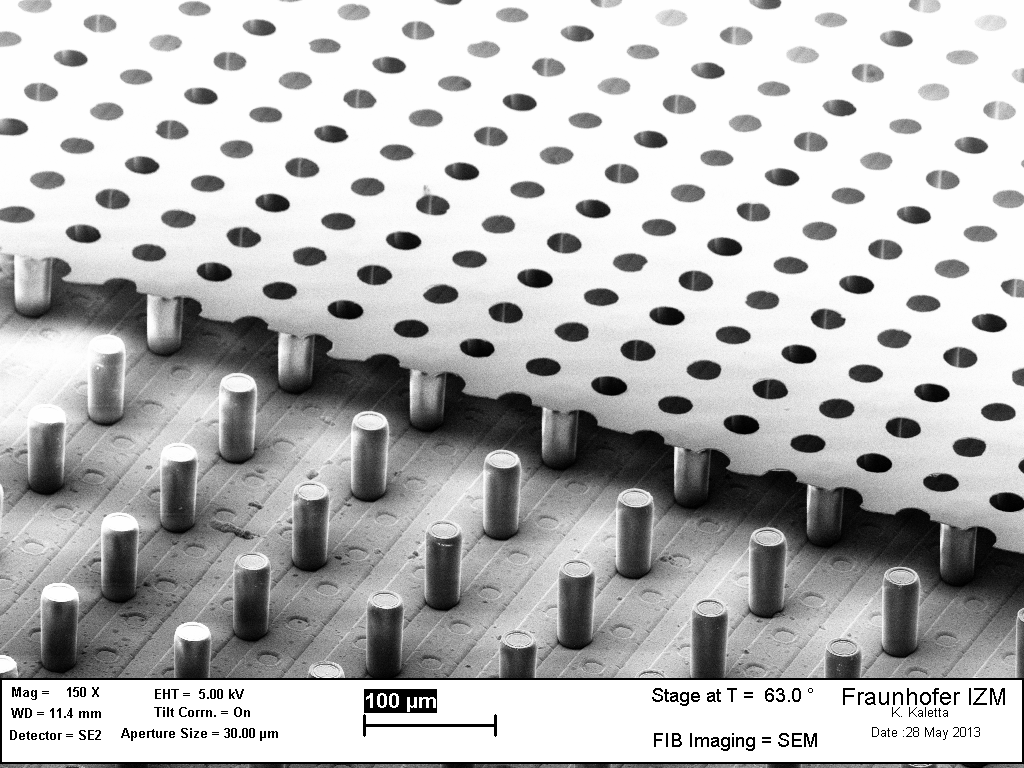
\includegraphics[width=\textwidth]{Tracker/TPC/GridPixes}
		\caption{GridPix detector with a partially removed grid}
		\label{fig:TPC:GridPix:GridPix}
	\end{minipage}
	\hfill
	\begin{minipage}{.49\textwidth}
		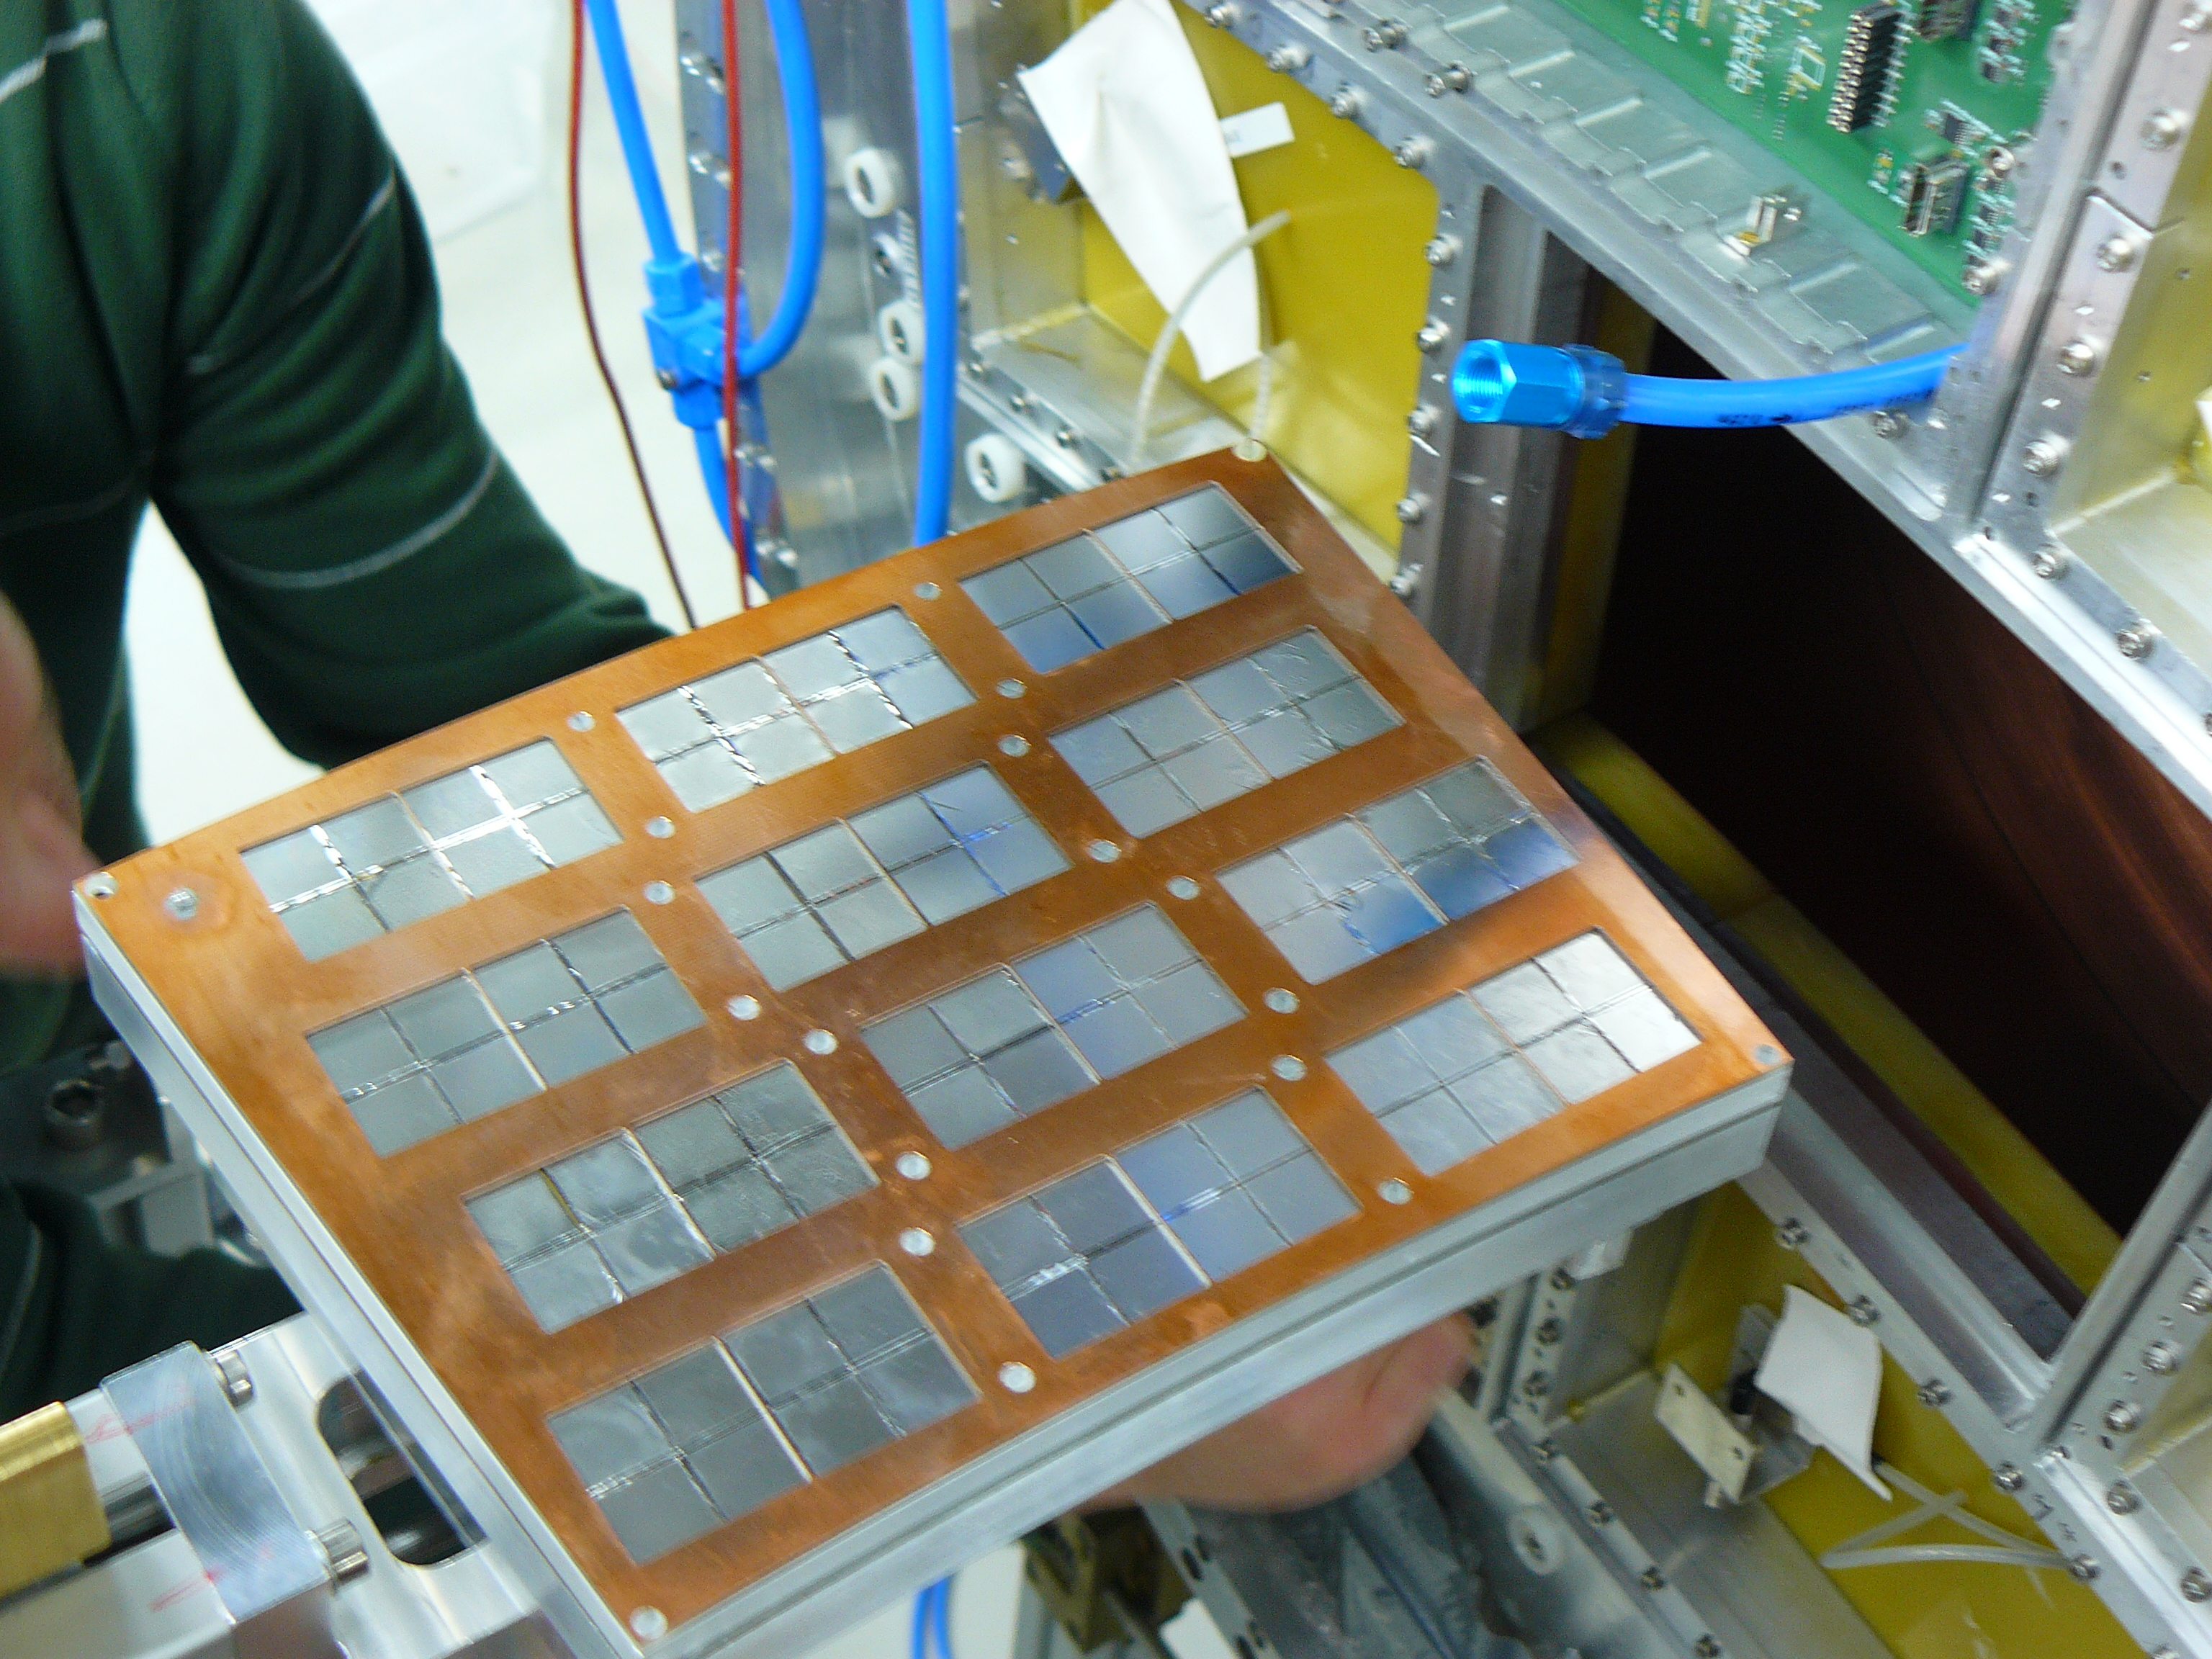
\includegraphics[width=\textwidth]{Tracker/TPC/FullModule}
		\caption{Fully equipped module as it is being mounted}
		\label{fig:TPC:GridPix:module}
	\end{minipage}
\end{figure}

\begin{figure}
	\begin{minipage}{.49\textwidth}
		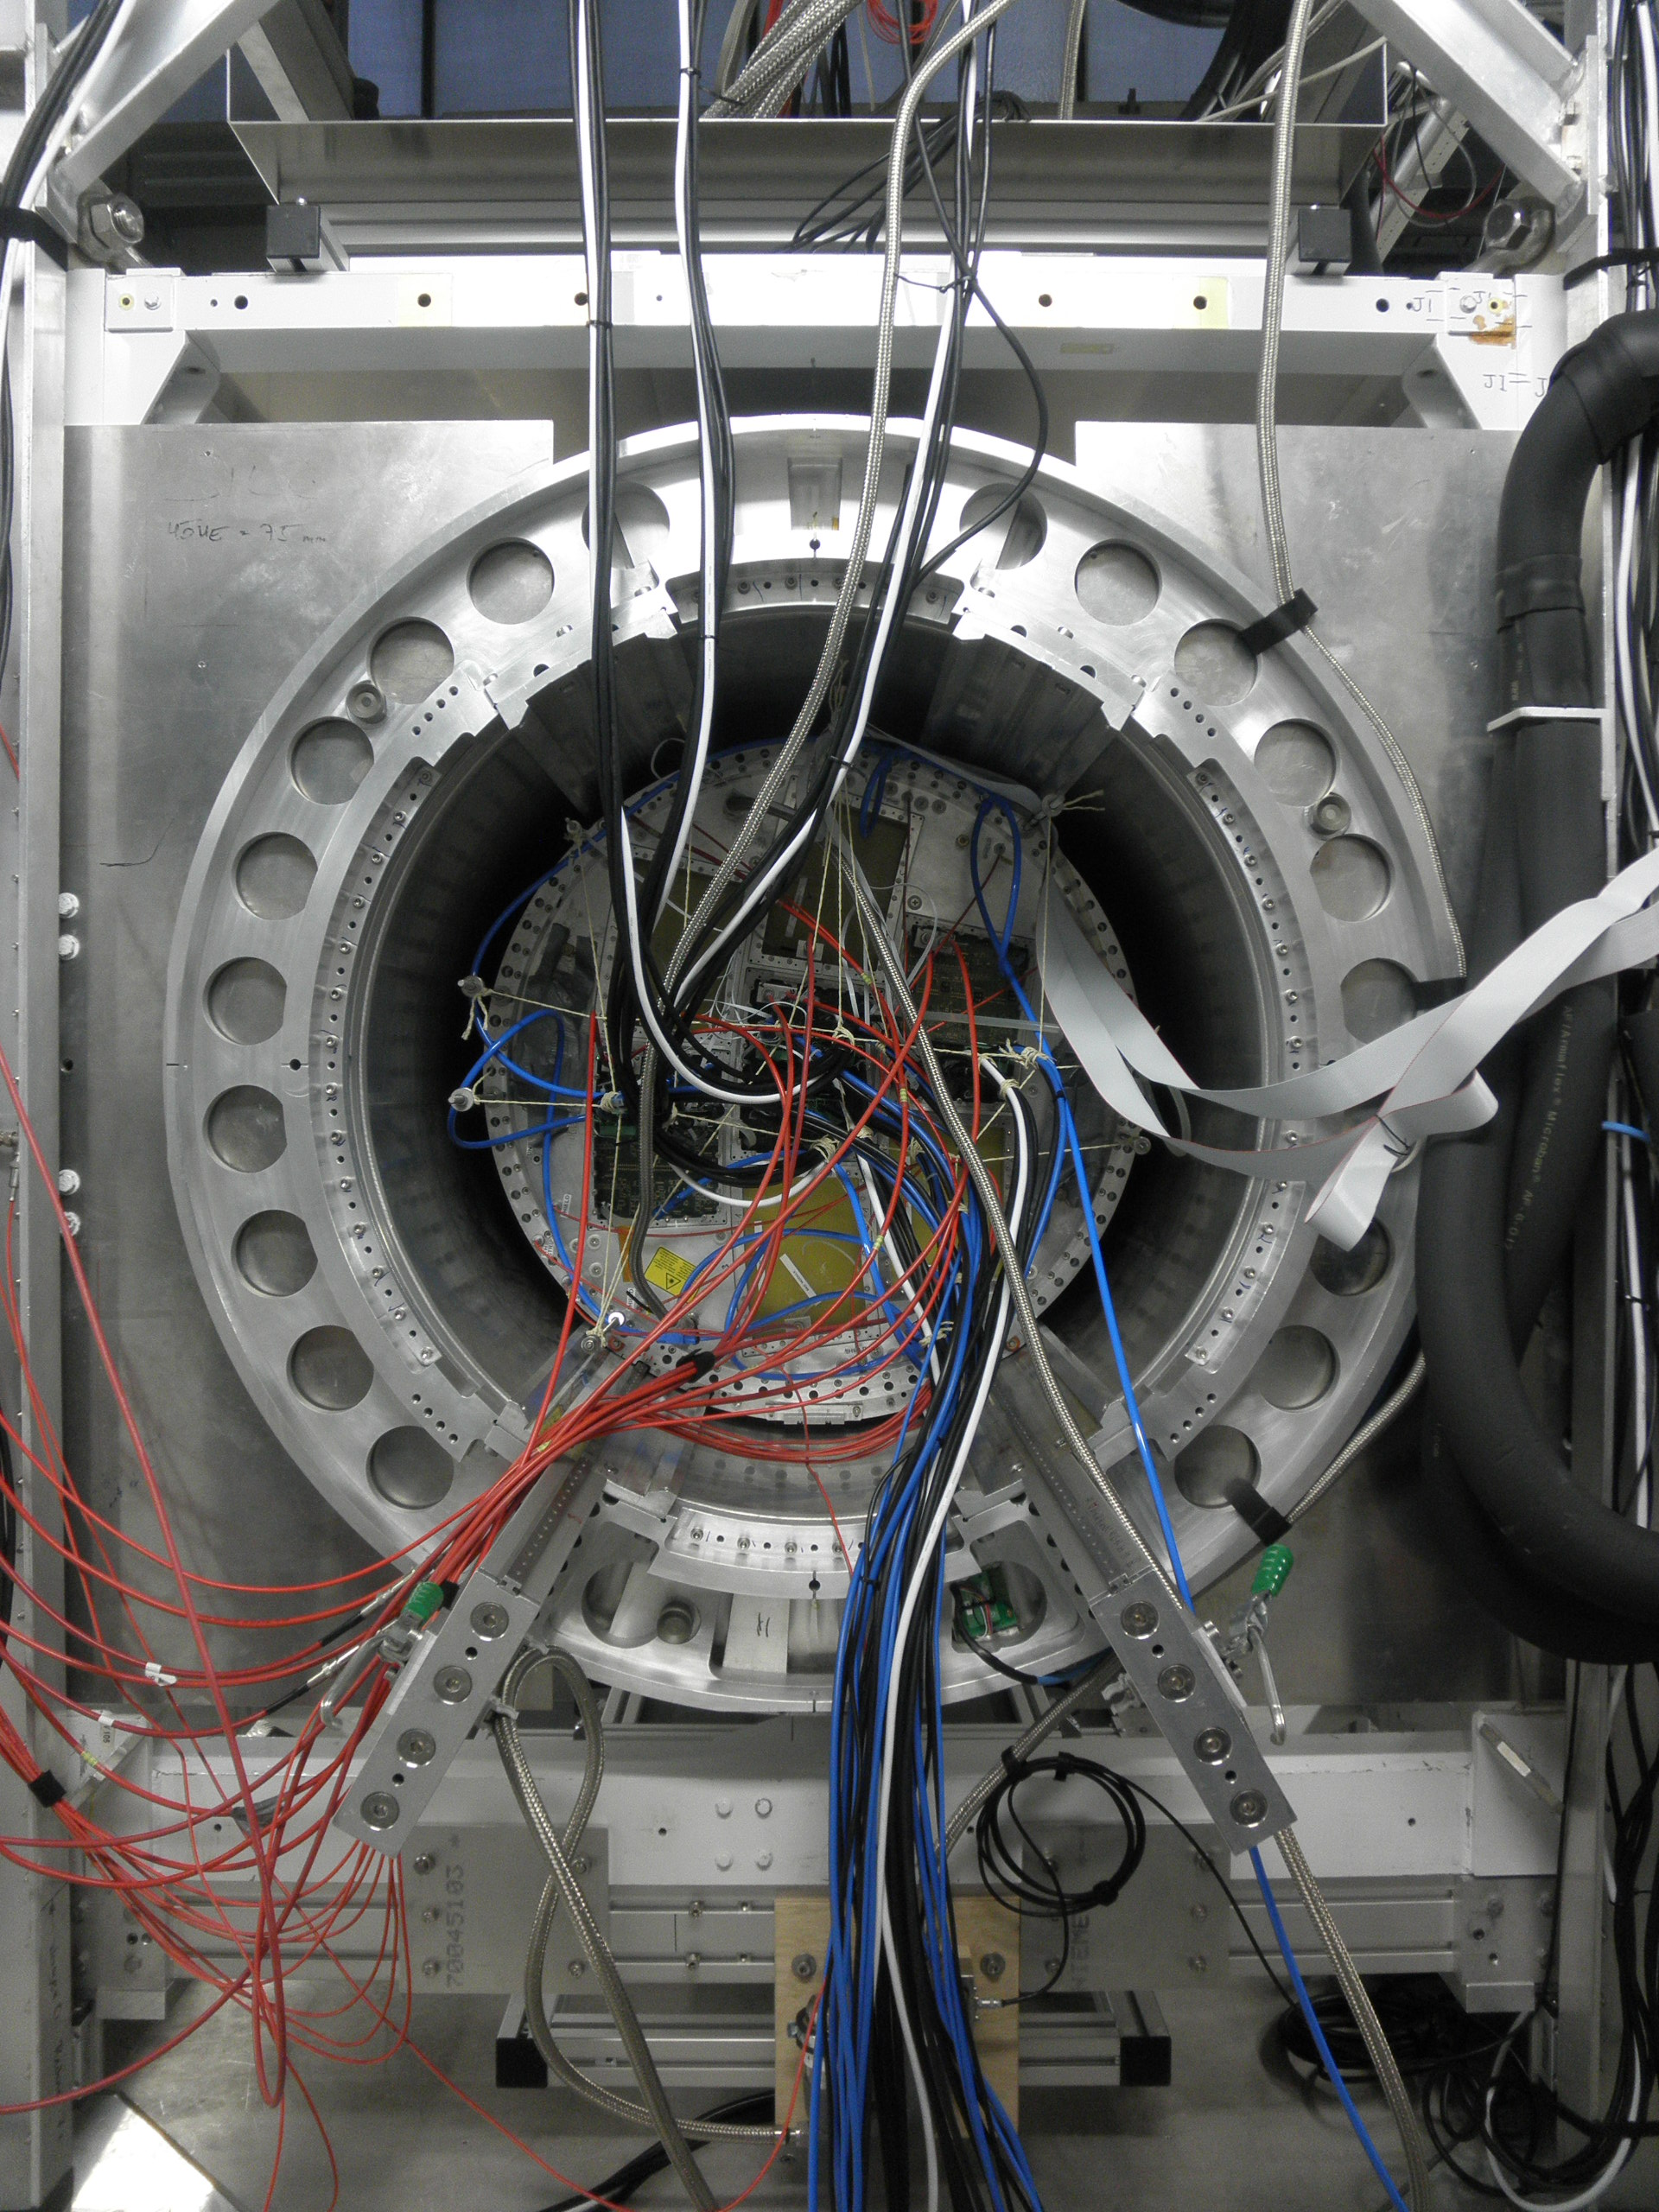
\includegraphics[width=\textwidth]{Tracker/TPC/Endplate_cabled}
		\caption{Fully cabled end plate}
		\label{fig:TPC:GridPix:endPlate}
	\end{minipage}
	\hfill
	\begin{minipage}{.49\textwidth}
		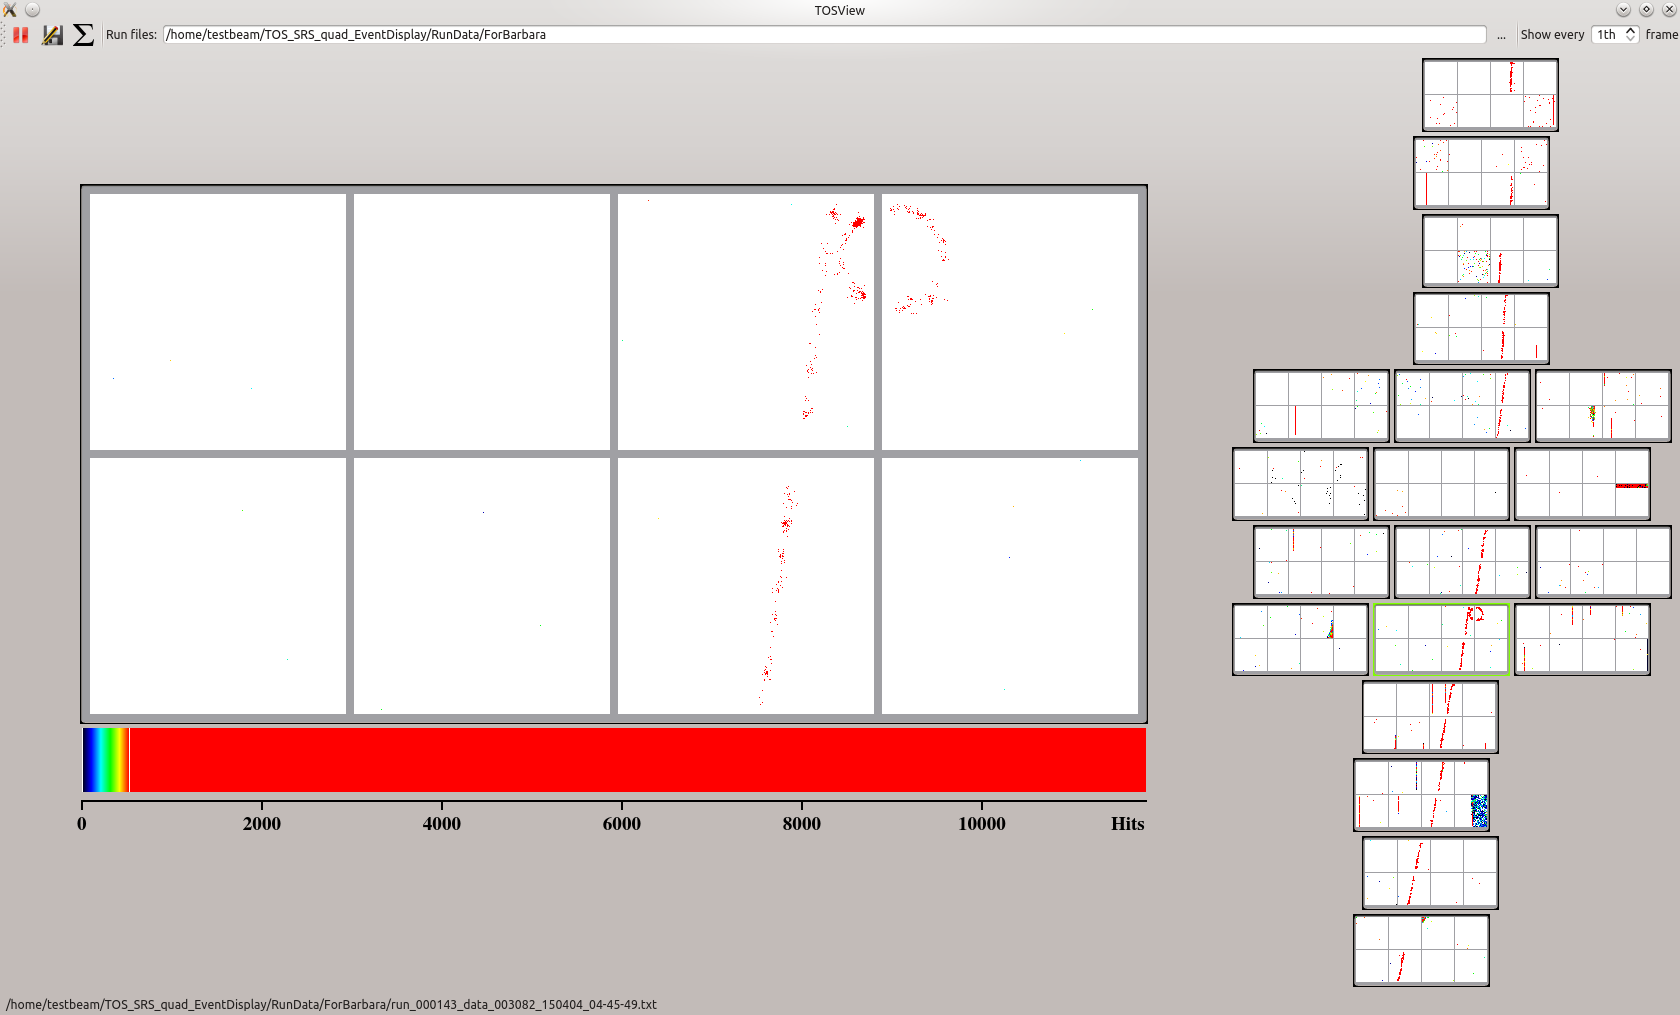
\includegraphics[width=\textwidth]{Tracker/TPC/onlineTrack}
		\caption{Online display of an example track}
		\label{fig:TPC:GridPix:onlineTrack}
	\end{minipage}
\end{figure}

\subsection{Engineering Challenges}
The production of a module with 160 GridPixes requires 4 main components:
\begin{enumerate}
	\item The production of a large number of GridPixes with sufficiently good quality. This has been addressed by the new production method, which is based on complete wafers. The process was developed in collaboration wit the Fraunhofer institute IZM a Berlin and yields up to 400 GridPixes per batch. Figure~\ref{fig:TPC:GridPix:GridPix} shows a GridPix detector with a partially removed grid.
	\item The challenge of the readout is being addressed by the new readout system as described above.
	\item The distribution of the LV power to all ASICs which can reach peek values of \unit[85]{A} at \unit[2.2]{V} was studied in a Master thesis.
	\item Cooling of the ASICs was done by cold water.
\end{enumerate}


\subsection{Future Plans}
Currently, the main focus is on the analysis of the test beam data. The challenge of finding and fitting tracks with several thousand hits is quite different from the standard pad-based TPC analysis. On a longer term all participating institutes are working on software to simulate, reconstruct and analyze data of the ILD-TPC (i.e. about 10,000 hits per track) so that the difference in performance between a pad and a pixel-based TPC can be studied.
On the hardware side we are interested in replacing the Timepix ASIC by the Timepix3 ASIC and produce GridPix detectors with this improved chip, which promises a much better performance, since it is multi-hit capable, can record both time and charge of a each signal and has a much faster digitization frequency. There are also some ideas of how to improve the grid structure and make it more reliable.

\subsection{Applications Outside of Linear Colliders}
A single InGrid detector will be installed this year in the CAST experiment for axion search. For a TPC in a CLIC detector, a highly granular (i.e. pixelized) readout structure is mandatory to lower the occupancy.
